
\section{Estimated limits on a light CP-odd scalar}
\label{sec:limit}

Following the analyses steps and the limit setting outlined in Sects.~\ref{sec:model}-\ref{sec:analysis}, we estimate expected 95\% CL upper limits
on the production cross section times branching ratio, $\sigma(\ttbar A) \times {\cal B}(A\to b\bar{b})$, as a function of $m_A$ (see Fig.~\ref{fig:limit_plots}).
Table~\ref{tab:sigma_95CL} summarises the 95\% CL upper limits on $\sigma(\ttbar A) \times {\cal B}(A\to b\bar{b})$ as a function of $m_A$ for different values
of the integrated luminosity. Under the assumption ${\cal B}(A\to b\bar{b})=1$, the upper limits on $\sigma(\ttbar A) \times {\cal B}(A\to b\bar{b})$ 
can be translated on upper limits on $|g_t|$, which are summarised in Table~\ref{tab:ct_95CL}.

Using the reconstruction strategy outlined in Sec.~\ref{subsec:analysis}, a CP-odd scalar that couples with $g_t=1$ can be excluded for $20 \leq m_A \leq 90$ GeV with only $30~\mathrm{fb}^{-1}$ of data (see Fig.~\ref{fig:limit_plots}). With an increased statistics of $300~\mathrm{fb}^{-1}$ couplings as low as $g_t \simeq 0.5$ can be constrained over a large mass range, i.e. $30 \leq m_A \leq 80$ GeV.

%%%%%%%%%%%%%%%%%%%%%%%%%%%%%%%%%%%%%%%%
\begin{figure}[htbp]
\begin{center}
\begin{tabular}{cc}
\includegraphics[width=0.45\textwidth]{Figures/BrasilianPlots/TTA_14_30.eps} &
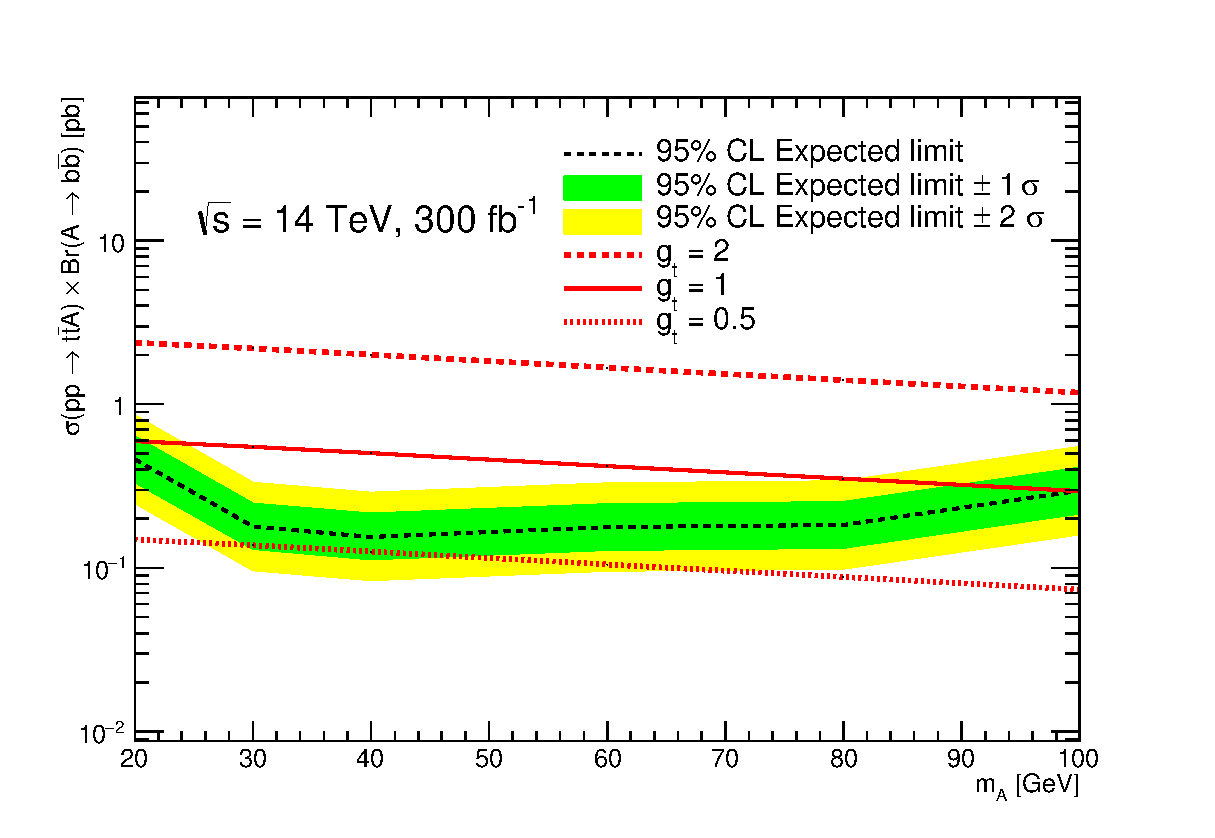
\includegraphics[width=0.45\textwidth]{Figures/BrasilianPlots/TTA_14_300.eps} \\
(a) & (b) \\
\end{tabular}
\caption{\small {Expected 95\% CL upper limits on $\sigma(\ttbar A) \times {\cal B}(A\to b\bar{b})$ as a function of $m_A$ 
in $pp$ collisions at $\sqrt{s}=14$ TeV for an integrated luminosity of (a) 30 fb$^{-1}$ and (b) 300 fb$^{-1}$. 
The green and yellow bands correspond to 1 and 2 standard deviations respectively around the median expected limit 
under the background-only hypothesis. Also shown are the theoretical cross sections for $\sigma(\ttbar A)$ for different  
assumed values of $g_t$ (0.5, 1.0 and 2.0) and ${\cal B}(A\to b\bar{b})=1$.}}
\label{fig:limit_plots}
\end{center}
\end{figure}
%%%%%%%%%%%%%%%%%%%%%%%%%%%%%%%%%%%%%%%%%%%%%%%%%%% 

%%%%%%%%%%%%%%%%%%%%%%%%%%%%%%%%%%%%%%%
\begin{table}[h] 
\begin{center} 
\begin{tabular}{ccccccc} 
\hline\hline
 & \multicolumn{6}{c}{95\% CL upper limits on $\sigma(\ttbar A) \times {\cal B}(A\to b\bar{b})$ (pb)} \\
\hline
  & \multicolumn{6}{c}{$m_A$ (GeV)} \\
  \cline{2-7} 
${\cal L}$ (fb$^{-1}$) & $\quad$ 20 $\quad$ & $\quad$ 30 $\quad$ & $\quad$ 40 $\quad$ & $\quad$ 60 $\quad$ & $\quad$ 80 $\quad$ & $\quad$ 100 $\quad$ \\
\hline
1 & 4.46 & 2.50 & 2.38 & 2.57 & 2.78 & 3.94 \\
30 & 1.02 & 0.48 & 0.45 & 0.51 & 0.53 & 0.78  \\
100 & 0.67 & 0.29 & 0.25 & 0.29 & 0.30 & 0.46 \\
300 & 0.46 & 0.18 & 0.16 & 0.18 & 0.18 & 0.30 \\
3000 & 0.17 & 0.066 & 0.057 & 0.065 & 0.065 & 0.13 \\
\hline\hline
\end{tabular} 
\caption{\small {Expected 95\% CL upper limits on $\sigma(\ttbar A) \times {\cal B}(A\to b\bar{b})$ as a function of $m_A$ 
in $pp$ collisions at $\sqrt{s}=14$ TeV for different integrated luminosities.}}
\label{tab:sigma_95CL} 
\end{center} 
\end{table} 
%%%%%%%%%%%%%%%%%%%%%%%%%%%%%%%%%%%%%%%

%%%%%%%%%%%%%%%%%%%%%%%%%%%%%%%%%%%%%%%
\begin{table}[h!] 
\begin{center} 
\begin{tabular}{ccccccc} 
\hline\hline
 & \multicolumn{6}{c}{95\% CL upper limits on $|g_t|$} \\
\hline
  & \multicolumn{6}{c}{$m_A$ (GeV)} \\
  \cline{2-7} 
${\cal L}$ (fb$^{-1}$) & $\quad$ 20 $\quad$ & $\quad$ 30 $\quad$ & $\quad$ 40 $\quad$ & $\quad$ 60 $\quad$ & $\quad$ 80 $\quad$ & $\quad$ 100 $\quad$ \\
\hline
1 & 2.73  & 2.14 & 2.18 & 2.48 & 2.82 & 3.65 \\
30 & 1.31  & 0.94 & 0.95 & 1.10 & 1.23 & 1.62 \\
100 & 1.06 & 0.72 & 0.71 & 0.83 & 0.93 & 1.25 \\
300 & 0.88 & 0.57 & 0.55 & 0.65 & 0.72 & 1.00 \\
3000 & 0.54 & 0.35 & 0.34 & 0.39 & 0.43 & 0.67 \\
\hline\hline
\end{tabular} 
\caption{\small {Expected 95\% CL upper limits on $|g_t|$ as a function of $m_A$ 
in $pp$ collisions at $\sqrt{s}=14$ TeV for different integrated luminosities, under the assumption ${\cal B}(A\to b\bar{b})=1$.}}
\label{tab:ct_95CL} 
\end{center} 
\end{table} 
%%%%%%%%%%%%%%%%%%%%%%%%%%%%%%%%%%%%%%%

